% !TEX root = ../thesis.tex

\chapter{Conclusion}
\label{chap:conclusion}

\cleanchapterquote{“Knowledge is just opinion that you trust enough to act upon.}{Orson Scott Card}{(Children of the Mind)}


% ------------------------------------------------------------------------------

In Chapter~\ref{chap:theory}, we saw multi-layer feedforward neural networks are universal approximators.
A sufficiently big fully-connected network could, theoretically, solve arbitrarily complex problems.
However, beyond some successes of convolutional neural networks in the late 1990's enabled by their reduction in the number of required learnable parameters, limited computational resources and training datasets hindered their use for solving real-world tasks.
The limitations of convolutional neural networks faded with the advent of general-purpose graphical processing units (CPGPUs) and the availability of large training datasets, sometimes complemented by huge unlabeled datasets used for unsupervised pre-training.
Deep neural networks are often used today, as they learn increasingly abstract notions from raw inputs.
Traditionally, pattern recognition algorithms required domain features to be carefully crafted by domain experts, but Deep Learning techniques carry out feature engineering automatically for us.

In Chapter~\ref{chap:context}, we reviewed how the feature extraction capabilities of deep neural networks outperformed existing techniques in object recognition challenges.
It is remarkable how well we understand how to make neural networks work for object recognition, as they now rival human performance in many aspects, especially when compared to how little we know about how they reason around highly-abstracted visual concepts once they are trained.
In an effort to understand the inner workings of deep neural networks, recent techniques try to visualize their internal representation of abstract concepts and have produced very intriguing images with with potential artistic implications.

In Chapter~\ref{chap:system}, we presented the Neural Style algorithm and how it managed to solve a long-standing problem in artistic rendering: the separation of style and content.
Whereas the algorithm can produce visually compelling compositions of style and content from two different source images, it requires fine-tuning on a per-case basis.
This limitation suggests that the Neural Style approach fails to grasp the notion of ``aesthetics'', which is another unsolved problem in artistic rendering, often studied in \emph{algorithmic aesthetics}.

In Chapter~\ref{chap:applications}, we surveyed a number of methods for improved style transfer and several other image processing problems that crucially depend on visual perception features.
Techniques based on deep convolutional networks have consistently outperformed state-of-the-art methods in their respective fields.

The separation of style and content is a very difficult problem to solve because it depends on human subjective perception of what style is and what content is in an artwork.
Formulating notions of ``aesthetics'' is a similarly complex problem, since we cannot formally define it and it totally builds upon human perception.

Capturing subjective opinions is currently being researched.
At the time of this writing, the Beauty.AI's First International Beauty Contest Judged by an Artificial Intelligence Jury \cite{YouthLaboratories} has already taken place.
Their promoters, supported by Nvidia and Microsoft among others, aim for teaching machines estimate human attractiveness by looking at the human face, relying for this on human-based perception.

In the light of the increasing interest in distilling inherently subjective features that are impractical to model formally, we find the study of aesthetics a relevant matter with practical applications.
Therefore, we believe the aesthetics of images could be similarly distilled and used for improving artistic rendering techniques.


% ------------------------------------------------------------------------------

\section{Future Work}
\label{sec:conclusion:future}

We propose further work on building an aesthetics-driven deep neural network for style transfer.
The system would consist of two sub-networks: one for image transformations and another for quality estimation.
The image transformation network, once trained, would produce perceptually-compelling images.
For training it, an aesthetic estimation network would rate the perceptual quality of the generated images and this estimate could be used as the loss function of the network.

Our first challenge is finding how to quantify the perceptual quality of an image.
In other words, modeling an inherently-subjective human notion.
For that we propose a convolutional neural network (CNN) that should be trained for estimating aesthetics based on human opinion.
The network could be either trained from scratch or based on a pre-trained network for object recognition, applying transfer learning techniques \cite{Pan2010}, which basically allow the network to adjust to a slightly different task or domain.

In order to train the aesthetics estimation network, we must have a sufficiently large and diverse training dataset of image-rating pairs.
We imagine a crowdsourcing platform with which to collect ratings from humans on artistic compositions.
People would be presented with two artistic images and they should decide which of the two images appeal them the most.
A similar work is currently being done in DeepArt.io's for the artistic Turing test (\url{https://turing.deepart.io/}).

The artistic images people would be rating could be composed of images from three sources: 1) a repository of classical paintings, 2) user-submitted style transfer creations, and 3) randomly-generated style transfer creations.
This last source would be generated from the repository of classical paintings, some repository of photographs, and randomly chosen style transfer hyperparameters.
Including them is of particular interest since it will result in more diverse, less biased artistic creations and, once ratings are collected, in a more representative training dataset for the aesthetic estimation network.

Important considerations to be taken into account when deploying the crowdsourcing initiative would be: acquiring a sufficiently large initial repository of images to rate, incentives to invite people to contribute, user interaction design to keep the contribution process simple, and, finally, potential partnerships with companies what could provide the computation facilities needed to run the initiative.

Our second challenge, once the aesthetic estimation network has been trained, is designing and training the image transformation network.
We have identified three plausible directions thus far.

Our first intuition is using a CNN whose very last layer is the Neural Style algorithm, as is.
The image transformation network in this case would learn how the Neural Style hyperparameters must be adjusted to produce a perceptually-compelling composition given a pair of source images.

Conversely, our second approach is keeping the Neural Style hyperparameters fixed.
In this case, the image transformation network would instead learn how to adjust the source images so that, when processed by Neural Style, the result would be appealing.

We anticipate two main problems with the previous approaches.
First, Neural Style is computationally expensive, as it requires backpropagation pass to produce every single image, and relying on it would terribly slow down the learning process.
And, second, we suspect reusing Neural Style as a black box layer would would unnecessarily constraint the learning process within the network.

To circumvent this, and inspired by \citeauthor{Johnson2016}'s approach \cite{Johnson2016}, we would completely disregard Neural Style in the image transformation network.
The network would learn how to maximize the perceived quality of a given style to photographs in a simple feedforward pass.
The question remains open whether the network could learn how to apply general style transfer given two images.
We conjecture, however, that, by using the aesthetics estimation network as part of the loss function, this could be possible.

We are confident such a system will not only be a versatile tool for artistic rendering but also for image processing in general.
Moreover, it might even be of great relevance to the advance of computational neuroscience, giving researchers a new way to look into how the creative process occurs in the human brain and which patterns in nature elicit the notion of beauty in our minds.

\vspace*{\fill}
{
  \begin{figure}[h]
    \setlength{\abovecaptionskip}{0pt}
    \captionsetup{
      font=bf,
      justification=centering,
      labelformat=empty
    }
    \begin{center}
      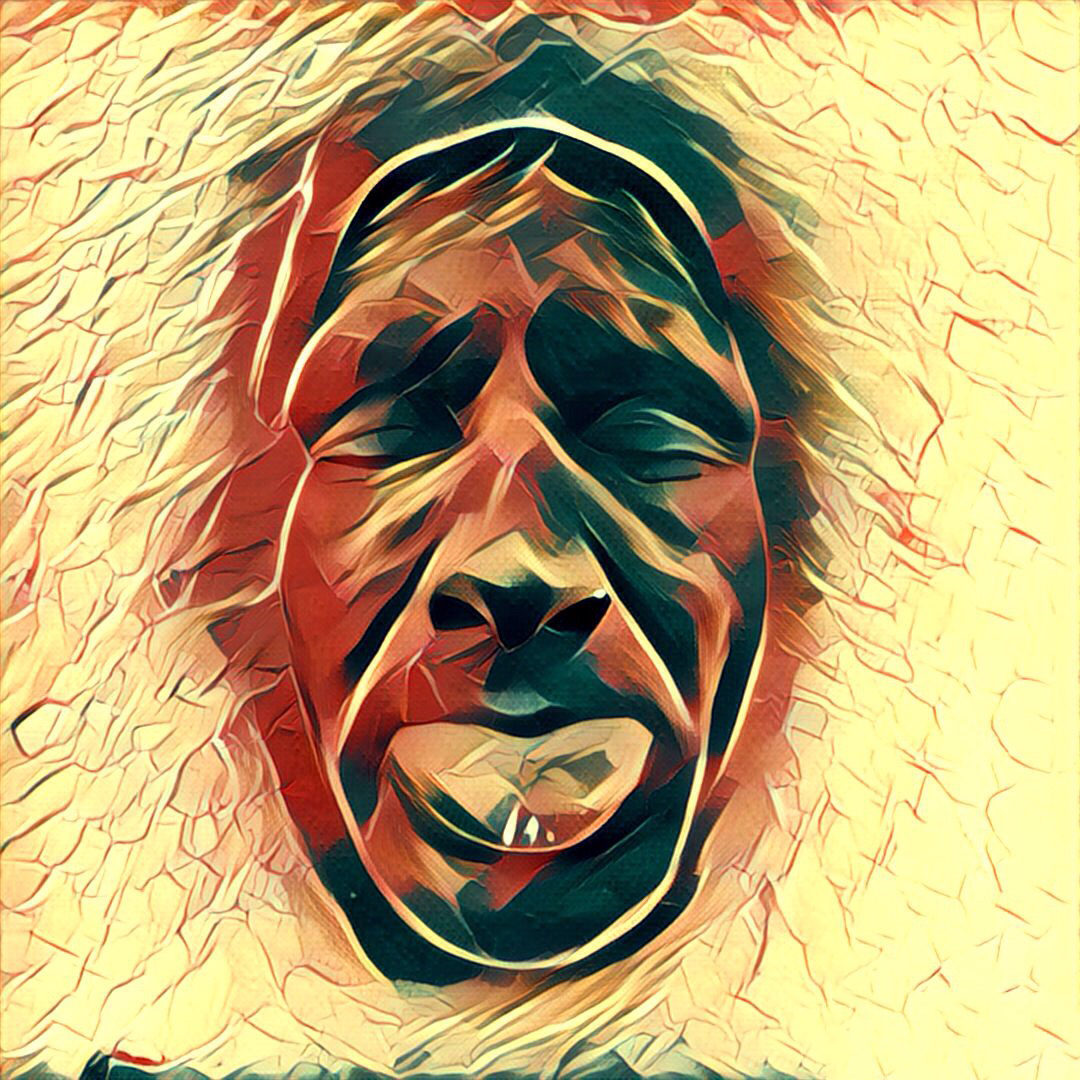
\includegraphics[width=0.5\textwidth]{gfx/prisma}
    \end{center}
    \caption{Form and Content}
  \end{figure}
}
\vspace*{\fill}
